\documentclass[11pt]{beamer}
\usetheme{Madrid}
\usepackage[utf8]{inputenc}
\usepackage[francais]{babel}
\usepackage[T1]{fontenc}
\usepackage{amsmath}
\usepackage{amsfonts}
\usepackage{amssymb}
\usepackage{graphicx}
\usepackage{tikz}
\title{Schémas Compact Hermitiens sur la Sphère\\
Séminaire Doctorants de Reims}
\setbeamercovered{transparent} 
%\setbeamertemplate{navigation symbols}{} 
\author{Brachet Matthieu}
\logo{IECL.jpg} 
\date[29.10.2015]{Vendredi 16 Octobre 2015}
\institute[IECL]{Institut Elie Cartan de Lorraine}
%\subject{} 
\begin{document}

\begin{frame}
\titlepage
\begin{center}

\includegraphics[width=2.5cm]{IECL.jpg}
\end{center}
\end{frame}

\begin{frame}
\tableofcontents
\end{frame}

% ********************************************************************************
\section{Introduction}
\begin{frame}{Introduction}

\begin{exampleblock}{Quoi?}
Calcul des opérateurs différentiels classiques sur la sphère par des méthodes numériques
\end{exampleblock}
\pause
\begin{exampleblock}{Pourquoi?}
Applications numériques en océanographie, climatologie, ...
\end{exampleblock}

\begin{figure}
\begin{center}
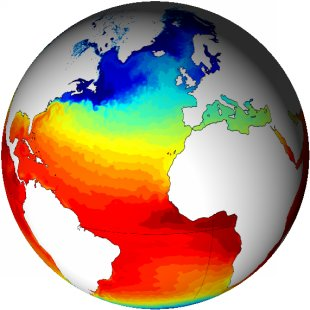
\includegraphics[height=3cm]{oceanographie.jpg}
\hspace{1cm}
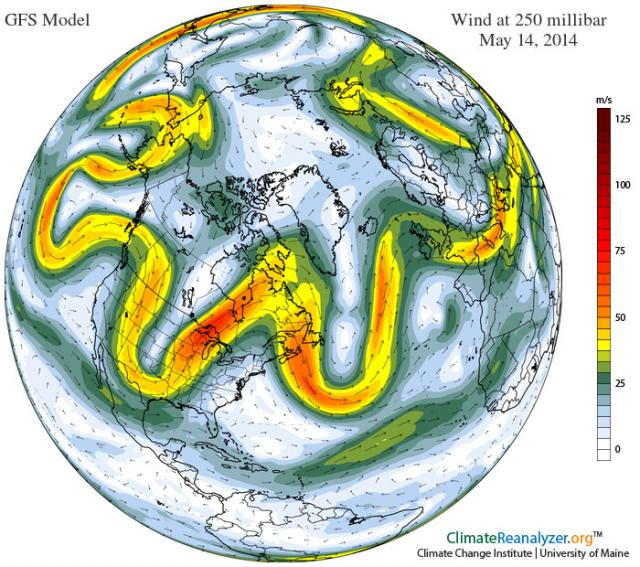
\includegraphics[height=3cm]{climato.jpg}
\end{center}
\caption{(a) Océanographie(Image Mercator océan) - (b) Jet-Stream (ClimateReanalyzer.org$^{TM}$)}
\end{figure}

\end{frame}

% ********************************************************************************

\section{Ce qui existe déjà...}
\begin{frame}
$\rightarrow$ \textbf{Maillage Longitude/Latitude}
\begin{columns}
\column{0.45\textwidth}
\begin{figure}
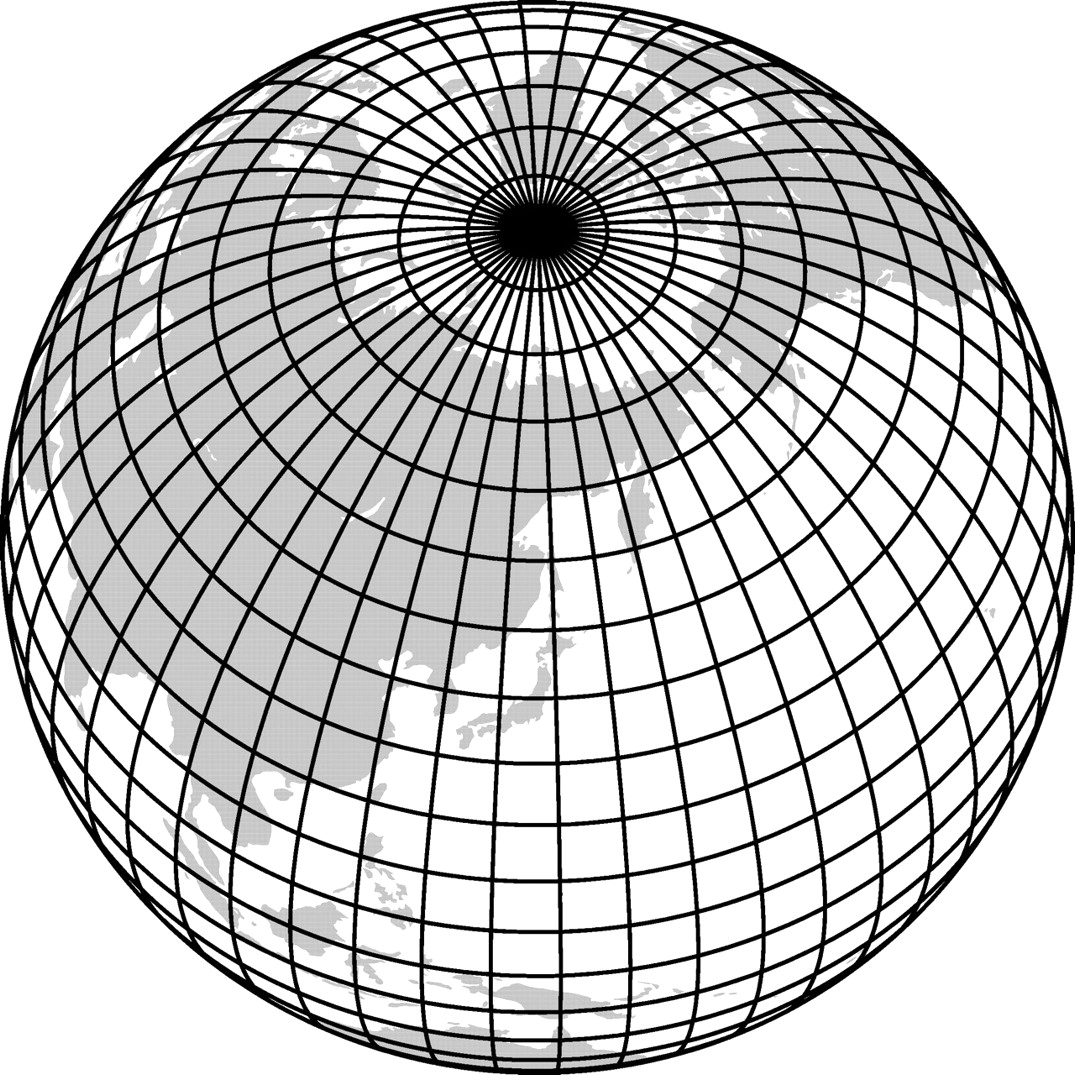
\includegraphics[height=3cm]{lonlat_grid.jpg}
\caption{Maillage Longitude/Latitude}
\end{figure}
\pause
\column{0.45\textwidth}
\begin{itemize}
\item Construction naturelle,
\item Facile à manipuler,
\item Problème des pôles.
\end{itemize}
\end{columns}
\end{frame}

\begin{frame}
$\rightarrow$ \textbf{Maillage Ying/Yang}

Introduit par Akira Kageyama et Tetsuya Sato en 2004.

\begin{columns}
\column{0.45\textwidth}
\begin{figure}
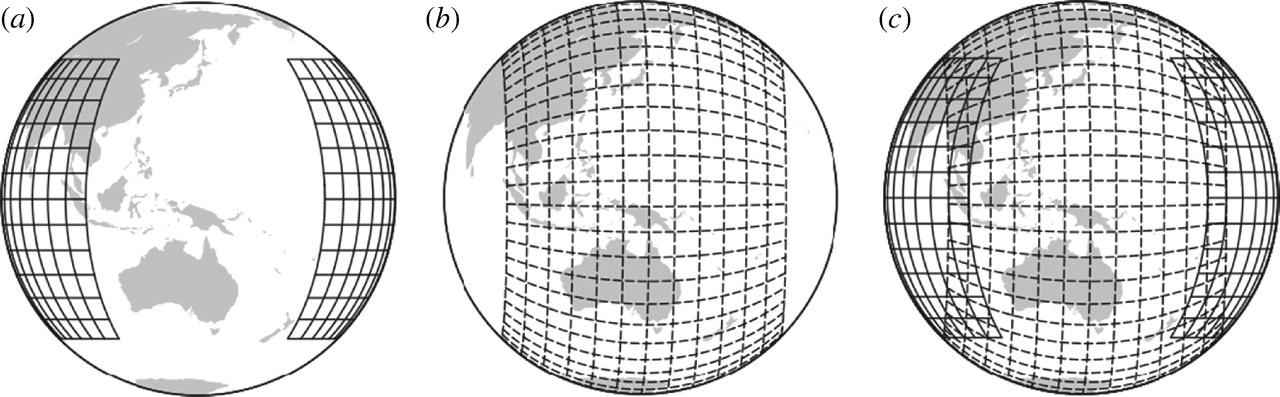
\includegraphics[width=6cm]{yingyang_grid.jpg}
\caption{Maillage Ying/Yang}
\end{figure}
\pause
\column{0.45\textwidth}
\begin{itemize}
\item Pas de problèmes de pôles,
\item Hautement parallèlisable,
\item Fort coût en calculs.
\end{itemize}
\end{columns}
\end{frame}

\begin{frame}
$\rightarrow$ \textbf{Maillage Isocahedrale}

Introduit par Robert Sadourny, Akio Arakawa et Yale Mintz en 1968.

\begin{columns}
\column{0.45\textwidth}
\begin{figure}
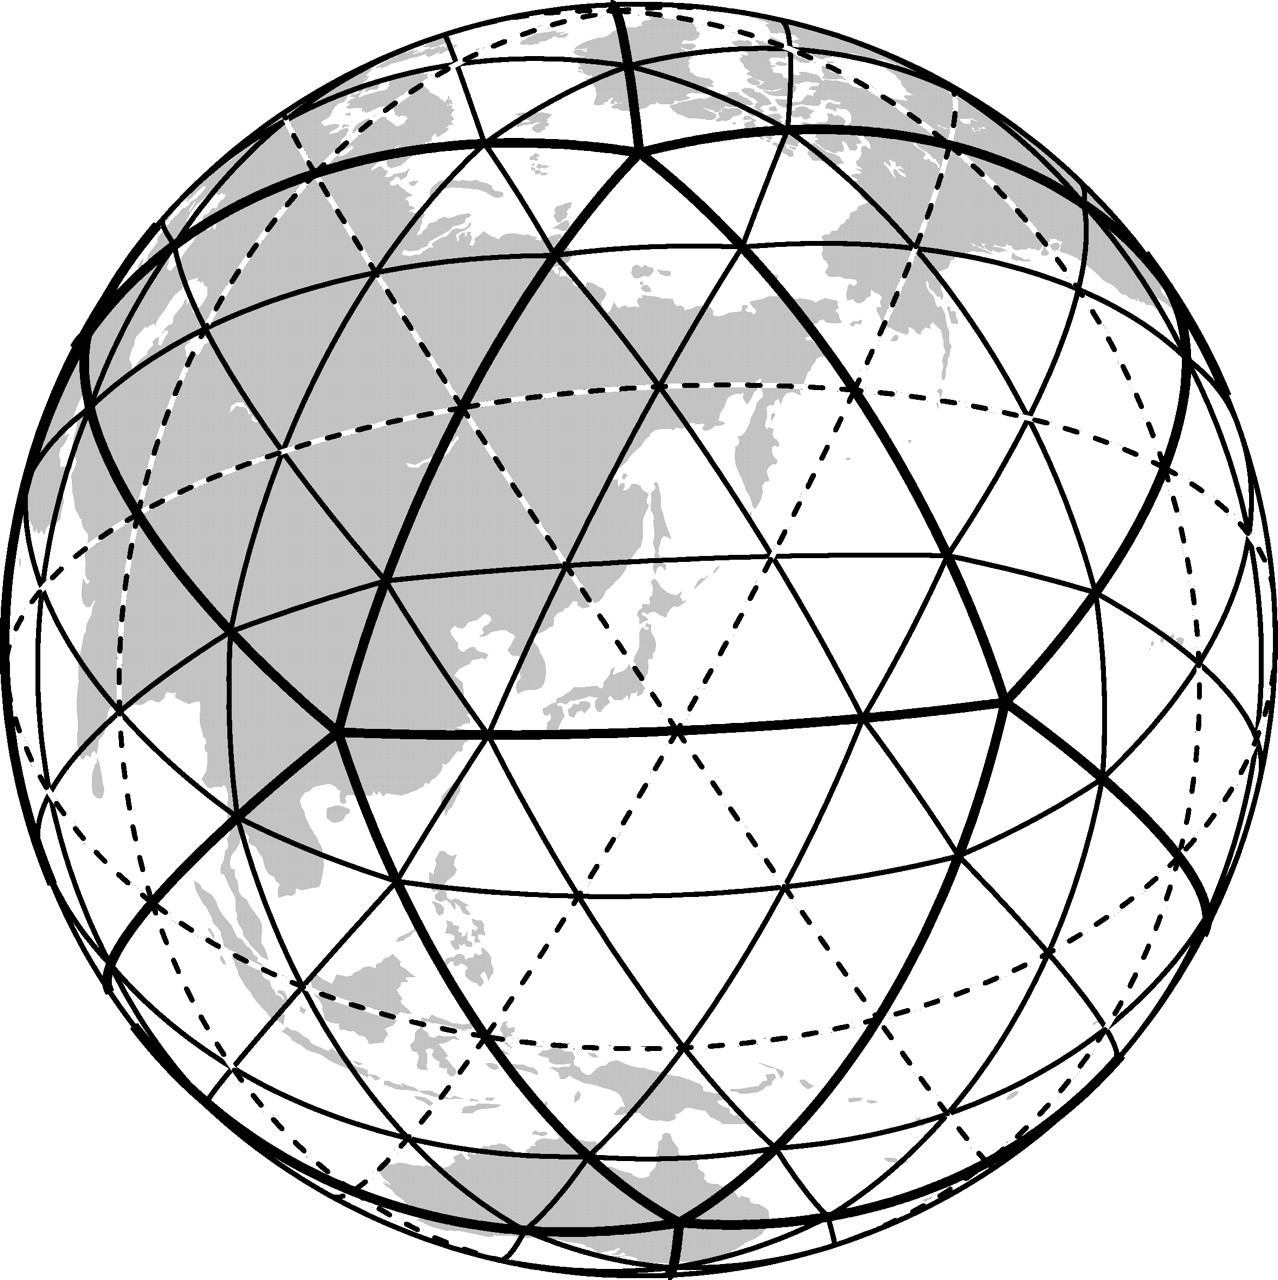
\includegraphics[height=3cm]{isocahedral_grid.jpg}
\caption{Maillage Isocahedrale}
\end{figure}
\pause
\column{0.45\textwidth}
\begin{itemize}
\item Coût en calcul faible,
\item Volume des éléments constant,
\item Problème des pôles toujours présent.
\end{itemize}
\end{columns}
\end{frame}



% ********************************************************************************
\section{Maillage "Cube-Sphere"}
\begin{frame}{Maillage "Cube-Sphere"}

\begin{exampleblock}{Idée :}
Construire une méthode rapide, précise et efficace pour calculer des opérateurs différentiels sur la sphère.
\end{exampleblock}

\pause

\begin{columns}

\column{0.45\textwidth}
Poles :
\begin{itemize}
\item Nord : $N (0,0,R)$,
\item Sud : $S (0,0,-R)$.
\end{itemize}

\begin{center}
\begin{tikzpicture}[scale=1.2]
    \draw (0,1) node {$\bullet$} ;
	\draw (0,1) node[above]{$N$} ;
	\draw (0,-1) node {$\bullet$} ;
	\draw (0,-1) node[below]{$S$} ;
    \draw (0,1) arc (90:270:0.75cm and 1cm);
    \draw (0,1) arc (90:270:0.50cm and 1cm);
    \draw (0,1) arc (90:270:0.25cm and 1cm);
    \draw (0,1) arc (90:270:0cm and 1cm);
    \draw (0,1) arc (90:-90:0.25cm and 1cm);
    \draw (0,1) arc (90:-90:0.50cm and 1cm);
    \draw (0,1) arc (90:-90:0.75cm and 1cm);    
    \draw (0,0) circle (1cm);
    \shade[ball color=blue!10!white,opacity=0.20] (0,0) circle (1cm);
\end{tikzpicture}
\end{center}

\pause

\column{0.45\textwidth}
Poles :
\begin{itemize}
\item East : $E (0,R,0)$,
\item West : $W (0,-R,0)$.
\end{itemize}
\begin{center}
\begin{tikzpicture}[scale=1.2]
	\draw (1,0) node {$\bullet$} ;
	\draw (1,0) node[right]{$E$} ;
	\draw (-1,0) node {$\bullet$} ;
	\draw (-1,0) node[left]{$W$} ;   
    \draw (-1,0) arc (180:360:1cm and 0.75cm);
    \draw (-1,0) arc (180:360:1cm and 0.25cm);
    \draw (-1,0) arc (180:360:1cm and 0.5cm);
    \draw (-1,0) arc (180:360:1cm and 0cm);
    \draw (-1,0) arc (180:360:1cm and -0.25cm);
    \draw (-1,0) arc (180:360:1cm and -0.5cm);
    \draw (-1,0) arc (180:360:1cm and -0.75cm);    
    \draw (0,0) circle (1cm);
    \shade[ball color=blue!10!white,opacity=0.20] (0,0) circle (1cm);
\end{tikzpicture}
\end{center}
\end{columns}
\end{frame}

\begin{frame}
\begin{exampleblock}{}
Création d'un maillage couvrant une partie de la sphère.
\end{exampleblock}
\begin{figure}
\begin{columns}
\column{0.45\textwidth}
\begin{center}
\begin{tikzpicture}[scale=1.2]
    \draw (-0.60,-0.60) arc (225:315:0.85cm and 0.50cm);
    \draw (-0.74,-0.17) arc (210:331:0.85cm and 0.16cm);
    \draw (-0.705,-0.35) arc (225:314:1cm and 0.5cm);
    \draw (-0.75,0) arc (180:360:0.75cm and 0cm);    
    \draw (0.74,0.17) arc (30:151:0.85cm and 0.16cm);
    \draw (0.705,0.35) arc (45:135:1cm and 0.5cm);
    \draw (0.60,0.60) arc (45:135:0.85cm and 0.50cm);
    \draw (0.60,-0.60) arc (-45:45:0.51cm and 0.85cm);
    \draw (0.17,-0.74) arc (-60:60:0.16cm and 0.85cm);
    \draw (0.35,-0.705) arc (-58:60:0.3cm and 0.82cm);
    \draw (0,0.75) arc (90:270:0cm and 0.75cm);
    \draw (-0.60,0.60) arc (135:225:0.51cm and 0.85cm);
    \draw (-0.17,0.74) arc (120:240:0.16cm and 0.85cm);
    \draw (-0.35,0.705) arc (122:240:0.3cm and 0.82cm);    
    \draw (0,0) circle (1cm);
    \draw (0.60,0.60) -- (0.707,0.707) ;
    \draw (-0.60,0.60) -- (-0.707,0.707) ;
    \draw (0.60,-0.60) -- (0.707,-0.707) ;
    \draw (-0.60,-0.60) -- (-0.707,-0.707) ;
    \shade[ball color=blue!10!white,opacity=0.20] (0,0) circle (1cm);
\end{tikzpicture}
\end{center}
\column{0.45\textwidth}
\begin{center}
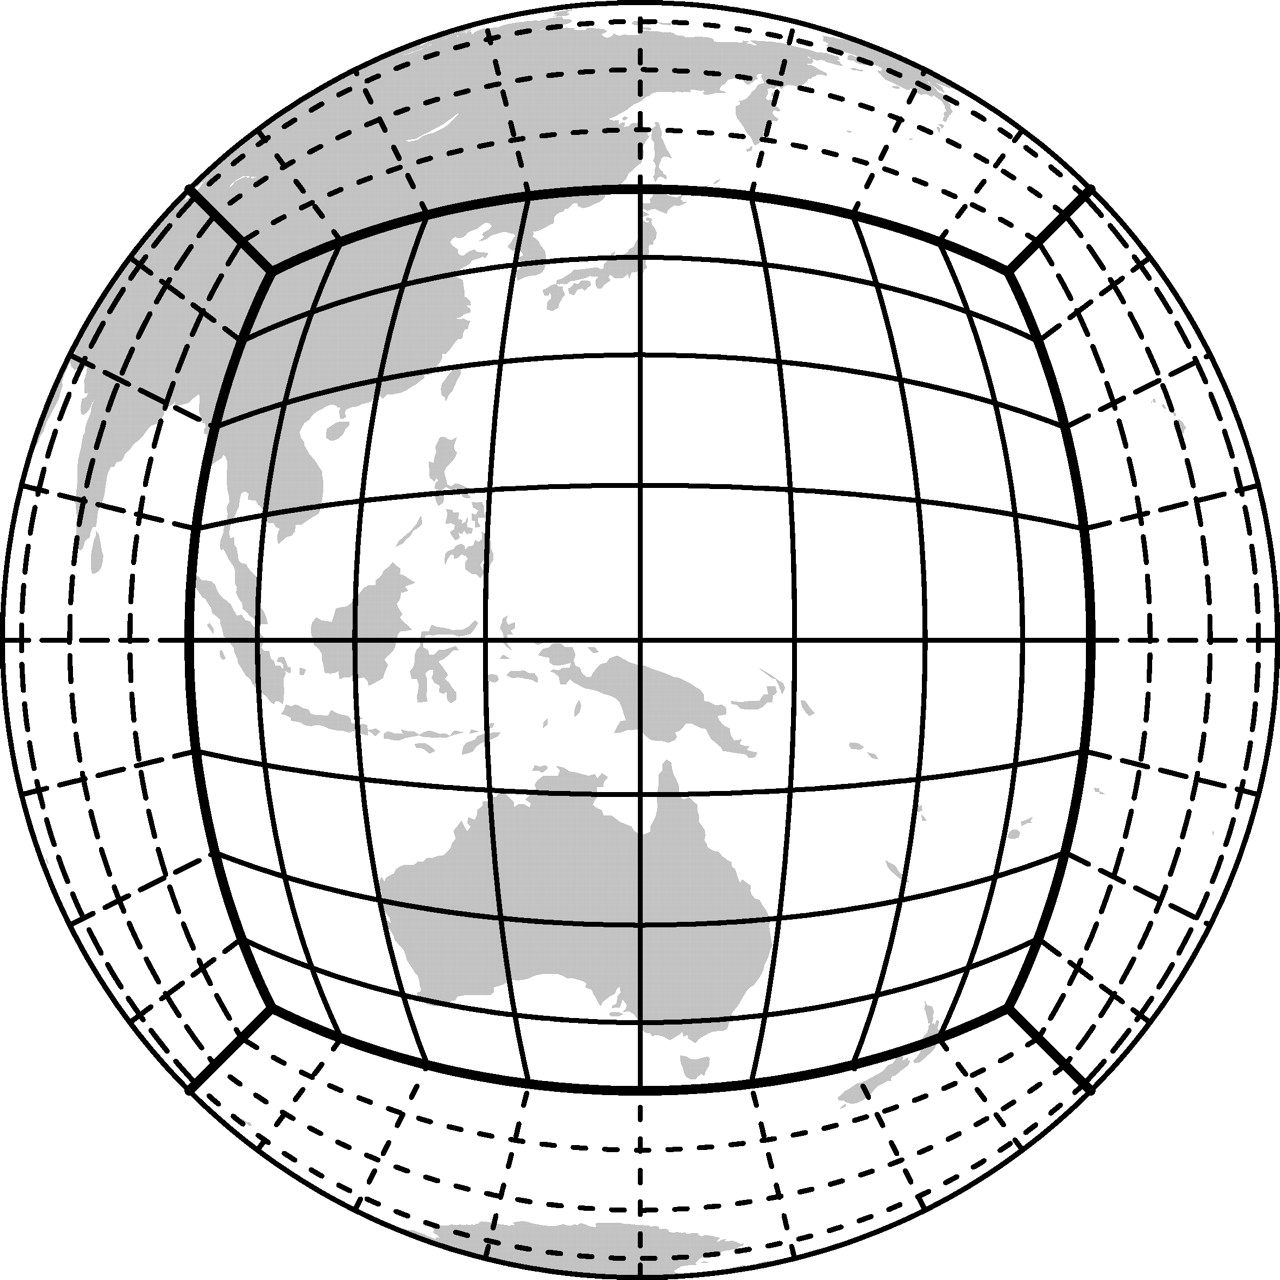
\includegraphics[scale=0.055]{CS_grid.jpg}
\end{center}
\end{columns}
\caption{Cube-Sphere - Front (gauche) et Complet (droite)}
\end{figure}
\end{frame}

% ********************************************************************************
\section{Calcul du gradient sphèrique}
\begin{frame}{Coordonnées}
\begin{columns}
\begin{column}{5cm}
\begin{figure}
\begin{tikzpicture}[scale=1.8]
	\draw (0,0) node {$\bullet$} ;
	\draw [>=stealth, ->] (0,0) -- (1.5,0) ; 
	\draw (1.5,0) node[above right]{$y$} ;   
	\draw [>=stealth, ->] (0,0) -- (1.1,-0.8) ; 
	\draw (1.1,-0.8) node[above right]{$x$} ; 
	\draw [>=stealth, ->] (0,0) -- (0,1.5) ; 
        \draw (0,1.5) node[above right]{$z$} ; 

        \draw[color=green] (0.065,0.5) arc (85:68:1cm and 0.5cm);
        \draw[color=green] (0.2,0.55) node{$\alpha$} ;
        \draw[color=red] (0.4,-0.05) arc (-5:25:0.41cm and 1cm);
        \draw[color=red] (0.48,0.2) node{$\beta$} ;
        \draw (-1,0)[dotted, color=black!40] arc (180:360:1cm and -0.5cm);
        \draw (0,1)[dotted, color=black!40] arc (90:270:-0.4cm and 1cm);
        \draw (-1,0)[dotted, color=black!20] arc (180:360:1cm and 0.5cm);
        \draw (0,1)[dotted, color=black!20] arc (90:270:0.4cm and 1cm);
    
        \draw (-1,0) arc (180:360:1cm and 0.06cm);
        \draw (0,1) arc (90:270:-0.08cm and 1cm);
        \draw[dashed] (-1,0) arc (180:360:1cm and -0.06cm);
        \draw[dashed] (0,1) arc (90:270:0.08cm and 1cm);
    
        \draw (0.36,0.46) node {$\bullet$} ;
	\draw (0.36,0.46) node[above right]{$M$} ;
        \draw (0,0) circle (1cm);
    \shade[ball color=blue!10!white,opacity=0.20] (0,0) circle (1cm);
\end{tikzpicture}
\caption{Coordonnées sur la CS}
\end{figure}
\end{column}
\pause
\begin{column}{5cm}
Dans ce système de coordonnées $M$ est donné par :

\begin{itemize}
\item $\alpha$ abscisse curviligne le long du grand cercle "horizontal".

\item $\beta$ abscisse curviligne le long du grand cercle "vertical".

\item $\xi$ angle equatiorial partant du centre du patch.

\item $\eta$ angle latitudinal partant du centre du patch.
\end{itemize}
\end{column}
\end{columns}

\begin{exampleblock}{}
Création d'un maillage régulier pour $\xi$ et $\eta$
\end{exampleblock}

\end{frame}


\begin{frame}{Calcul du gradient sphèrique}
Gradient :
$$\nabla_T u = \dfrac{\partial u}{\partial \xi}_{|\eta} g^\xi + \dfrac{\partial u}{\partial \eta}_{|\xi} g^\eta $$

$\rightarrow$ $\dfrac{\partial u}{\partial \xi}_{|\eta}$ et $\dfrac{\partial u}{\partial \eta}_{|\xi}$ : pas le long des grands cercles. Exprimer dans $(\alpha, \beta)$.
\pause
\begin{block}{Gradient sur la CS}
$$\nabla_T u = \frac{\partial u}{\partial \alpha}_{|\eta} \left( \cos \eta \dfrac{1+ \tan^2 \xi}{1 + \cos^2 \eta \tan^2 \xi} \right) g^\xi + \frac{\partial u}{\partial \beta}_{|\xi} \left( \cos \xi \dfrac{1+ \tan^2 \eta}{1 + \cos^2 \xi \tan^2 \eta} \right) g^\eta $$
\end{block}
\pause
$\rightarrow$ Évaluer $\dfrac{\partial u}{\partial \alpha}_{|\eta}$ et $\dfrac{\partial u}{\partial \beta}_{|\xi}$ en chaque point du maillage.
\end{frame}


% ********************************************************************************
\section{Dérivées Hermitiennes}
\begin{frame}{Dérivées Hermitiennes}
$u$ assez régulière et périodique. Alors :

$$\dfrac{u(x+h)-u(x-h)}{2h} = u'(x) + \dfrac{h^2}{6} \underbrace{u^{(3)}(x)}_{= \left( u'(x) \right)''} + \mathcal{O}\left( h^4 \right)$$

\pause

$$\dfrac{u(x+h)-u(x-h)}{2h} = u'(x) + \dfrac{h^2}{6} \mathbf{ \dfrac{u'(x-h) - 2 u'(x) + u'(x+h) }{h^2}} + \mathcal{O}\left( h^4 \right)$$

\pause

\begin{block}{}
Après simplification :
$$\dfrac{u(x+h)-u(x-h)}{2h} = \dfrac{1}{6} \left[ u'(x-h) + 4 u'(x) + u'(x+h) \right] + \mathcal{O}\left( h^4 \right)$$
\end{block}
\end{frame}

\begin{frame}
\begin{block}{Schéma compact}
\begin{itemize}
\item $U' = \left[ u'_1, \hdots ,u'_N \right]^T \approx \left[ u'(x_1), \hdots ,u'(x_N) \right]^T$

\item $U = \left[ u_1, \hdots ,u_N \right]^T$
\end{itemize}

\pause

Alors :
$$\dfrac{1}{2h}\begin{pmatrix}
0 & 1 &   &   & -1 \\ 
-1 & 0 & 1 & (0) &   \\ 
  & \ddots & \ddots & \ddots &   \\ 
  & (0) & -1 & 0 & 1 \\ 
1 &   &   & -1 & 0
\end{pmatrix} U = \dfrac{1}{6} \begin{pmatrix}
4 & 1 &   &   & 1 \\ 
1 & 4 & 1 & (0) &   \\ 
  & \ddots & \ddots & \ddots &   \\ 
  & (0) & 1 & 4 & 1 \\ 
1 &   &   & 1 & 4
\end{pmatrix} U'$$
\end{block}
\pause
$\rightarrow$ Résolution d'un système linéaire sur chaque grand cercle.

$\rightarrow$ Existence d'un solveur rapide combinant l'algorithme de Thomas et la formule de Shermann-Morisson-Woodbury.
\end{frame}

% ********************************************************************************

\begin{frame}

  \begin{alertblock}{Problème...}
  Les points des cercles ne coïncident pas avec les points du maillage  
  \end{alertblock}
  
\begin{columns}
\column{0.45\textwidth}

\begin{figure}
\begin{center}
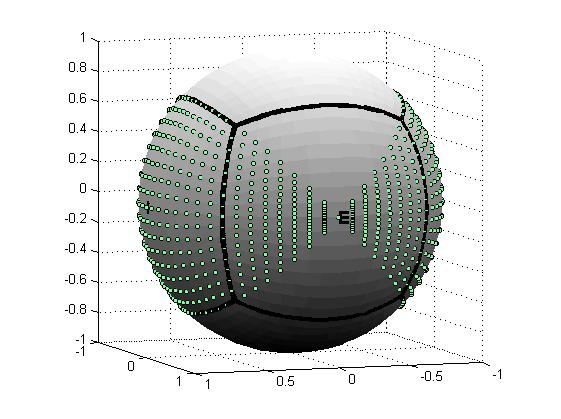
\includegraphics[height=3cm]{fig22.jpg}
\end{center}
\caption{grand cercle}
\end{figure}

\pause
\column{0.45\textwidth}

\begin{exampleblock}{Solution}
  \begin{itemize}
  \item Interpolation d'Hermite

    $\rightarrow$ Faible coût en calcul. \\
    $\rightarrow$ Phénomène de Runge... Grosse erreur due au grand nombre de points.

  \item Choix du spline cubique

    $\rightarrow$ Systèmes linéaires à résoudre.\\
    $\rightarrow$ Erreur en $\mathcal{O}\left( h^4 \right)$.
  \end{itemize}
\end{exampleblock}

\end{columns}

\end{frame}

% ********************************************************************************
\section{Benchmark}
\begin{frame}{Benchmark}
Résolution de :

$$\left\{
\begin{array}{rcl}
\dfrac{\partial h}{\partial t} + \mathbf{c} \cdot \nabla_S h & = & 0 \\
h(\mathbf{x},t=0) & = & h_0 ( \mathbf{x} )
\end{array}
\right. \hspace{1cm} \mathbf{x} \text{ sur la sphère, } t>0$$

\pause

\begin{block}{Discrétisation : }

\begin{itemize}
\item En espace : comme vu plus tôt,

\item En temps : méthode RK4 (ordre 4 et explicite) avec filtrage en espace des hautes fréquences (ordre 10).
\end{itemize}
\end{block}

\end{frame}

% ***

\begin{frame}{Test 1 : BUMP en rotation}
\begin{columns}
\column{0.45\textwidth}
Idée :

\begin{itemize}
\item $\mathbf{c}$ et $h_0$ donnés,

\item faire tourner une "cloche" (le BUMP) autour de la sphère.
\end{itemize}


\column{0.45\textwidth}

\begin{figure}
\href{run:CSapprox_test0.avi}{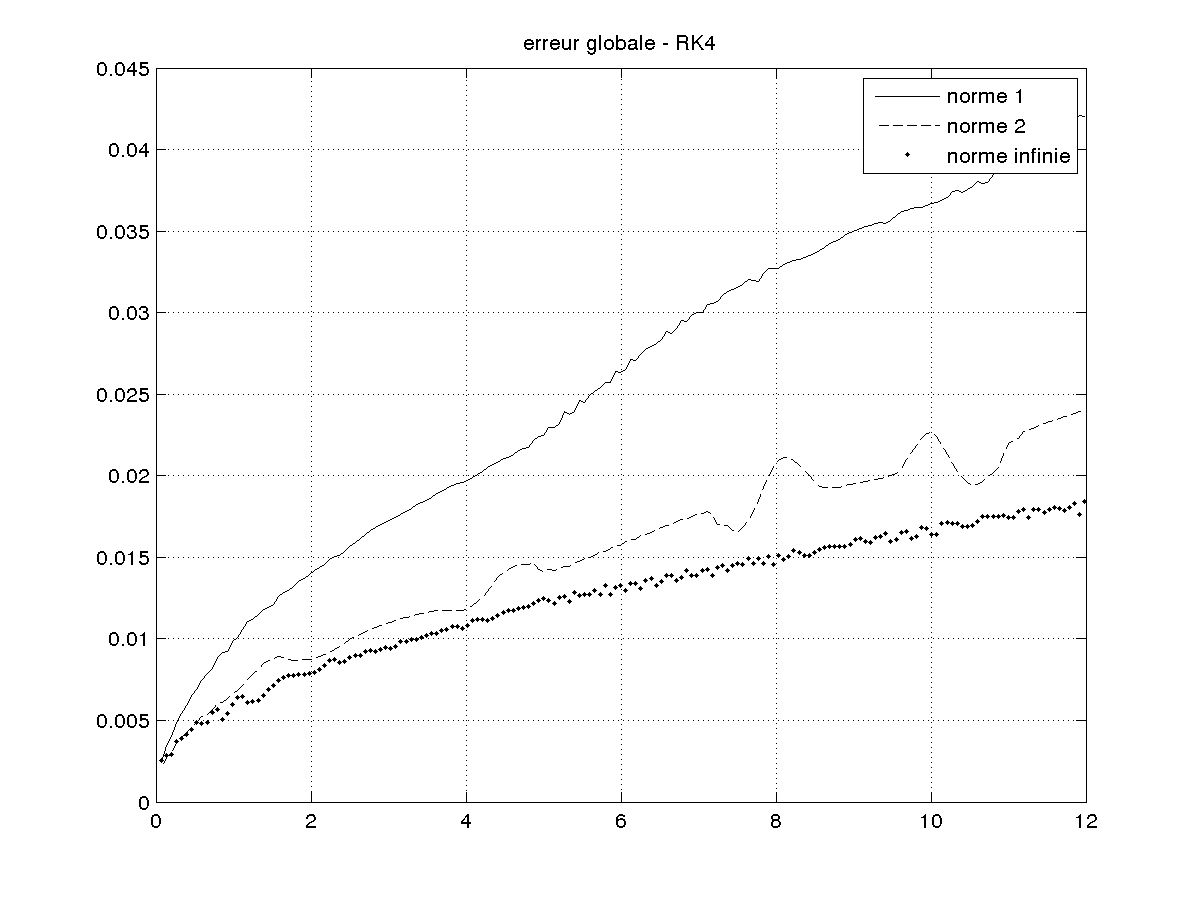
\includegraphics[scale=0.25]{normerreur_test0_100cfl90.png}} 
\caption{Test 1 : Bump en rotation - 40 mailles par face - CFL=0.9}
\end{figure}

\end{columns}
\end{frame}

% ***

\begin{frame}{Test 2 : Vortex stationnaire (Nair et Machenhauer - 2001}
\begin{columns}
\column{0.45\textwidth}
Idée :

\begin{itemize}
\item $\mathbf{c}$ et $h_0$ donnés,

\item Formation d'une "tempête" (vortex) sur une zone localisée de la sphère.
\end{itemize}


\column{0.45\textwidth}

\begin{figure}
\href{run:CSapprox_test1.avi}{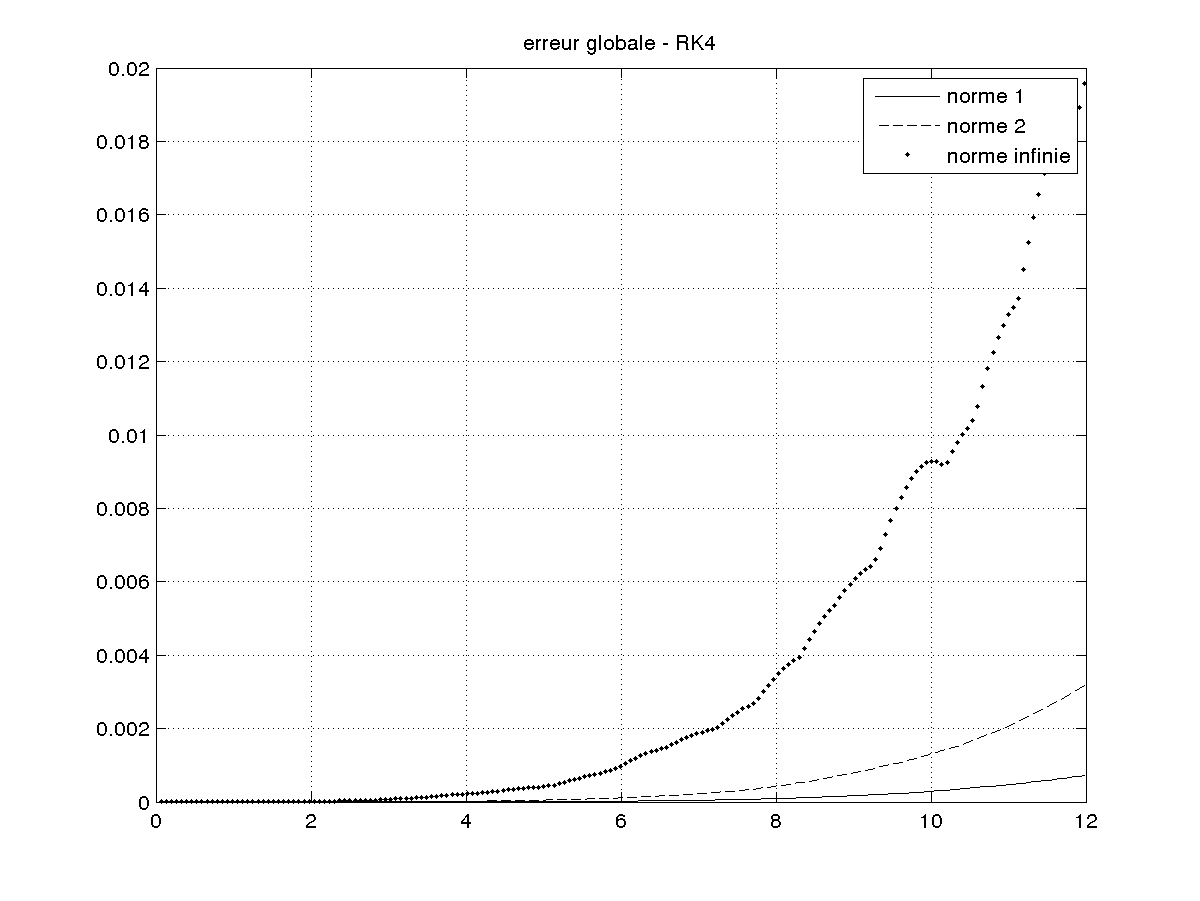
\includegraphics[scale=0.25]{normerreur_test1_100cfl90.png}} 
\caption{Test 2 : Vortex stationnaire - 40 mailles par face - CFL=0.9}
\end{figure}
\end{columns}
\end{frame}

% ***

\begin{frame}{Test 3 : Vortex instationnaire (Nair et Jablonowski - 2007)}
\begin{columns}
\column{0.45\textwidth}
Idée :

Combiner les deux tests précédents : test de déformation et de déplacement.
\begin{itemize}

\item $\mathbf{c}$ et $h_0$ donnés et issus des tests 1 et 2,

\item Formation d'une "tempête" (vortex) se déplacant le long d'un cercle sur la sphère.
\end{itemize}


\column{0.45\textwidth}

\begin{figure}
\href{run:CSapprox_test2.avi}{\includegraphics[scale=0.25]{14-Oct-2015_normerreur_test_2.png}} 
\caption{Test 3 : Vortex instationnaire - 40 mailles par face - CFL=0.9}
\end{figure}
\end{columns}
\end{frame}

\begin{frame}

Observation de l'erreur relative :

$$e_2^n = max_{\text{face}} \dfrac{ \| h^n_{i,j} - h(\mathbf{x}_{i,j}, t^n ) \|_2 }{\| h(\mathbf{x}_{i,j}, t^n ) \|_2}$$

\begin{figure}
\begin{tabular}{ccc}
Nombre de points par face & $max_n |e_2^n|$ & estimation de l'ordre \\
\hline
\hline
$41$ & $9.7386 (-2)$ & - \\
\hline 
$51$ & $5.0160 (-2)$ & $3.0399$ \\
\hline
$61$ & $2.6157 (-3)$ & $3.6365$ \\
\hline
$81$ & $8.3722 (-4)$ & $4.0173$ \\
\hline
$101$ & $3.4524 (-4)$ & $4.0143$\\
\hline
$151$ & $6.9199 (-5)$ & $3.9966$
\end{tabular}
\caption{Analyse de convergence du test 3 - $cfl = 0.7$}
\end{figure}

\end{frame}


% ********************************************************************************
\section{Conclusion et perspectives}
\begin{frame}{Conclusion et perspectives}
\begin{block}{Bilan}
\begin{itemize}
\item Méthode rapide (solveurs rapides) et précise (ordre 4),

\item Bons résultats sur les tests.
\end{itemize}
\end{block}

\pause

\begin{block}{Avenir...}
\begin{itemize}
\item Etude sur les harmoniques sphériques,

\item Mise en place d'un zoom LDC,

\item Résolution de l'équation de Saint-Venant.
\end{itemize}
\end{block}
\end{frame}

% ********************************************************************************

\begin{frame}
\frametitle{Bibliographie}

\begin{thebibliography}{9}
        

\scriptsize{

\bibitem{Lele}
         Sanjiva K. Lele
         \emph{: Compact Finite Difference Schemes with spectral-like resolution}.
         1991.

\bibitem{Croisille}
         J.-P. Croisille
         \emph{: Hermitian compact interpolation on the cubed-sphere grid}.
         2013.

\bibitem{Nair Jablonowski}
         Ramachandran D. Nair et Christiane Jablonowski
         \emph{: Moving Vortices on the Sphere : A test case for Horizontal Advection Problems}.
         1991.

\bibitem{Redonnet}
         Stéphane Redonnet
         \emph{: Simulation de la propagation acoustique en présence d'écoulements quelconques et de structures solides par résolution numérique des équations d'Euler}.
         Thèse, 2001.
         
\bibitem{Williamson}
         David L. Williamson, John B. Drake, James J. Hack, Rüdiger Jakob et Paul N.Swarztrauber
         \emph{: A strandard test set for Numerical Approximations to the Shallow Water Equations in Spherical Geometry}.
         1994.
    
    }     
         
         
         
\end{thebibliography}
\end{frame}

% ********************************************************************************
\begin{frame}
\begin{center}
Merci de votre attention :)
\end{center}
\end{frame}


\end{document}
